%!TeX root=./ordenacao.tex

%% ------------------------------------------------------------------------- %%


\section{Lista ordenada cinética}
\label{sec:lista}
Um jeito natural de resolver o problema da ordenação cinética é por
meio de uma lista ordenada cinética, que é manter um vetor com os
elementos dados em ordem decrescente do valor no instante atual.

Inicialmente o vetor começa com os valores dos elementos no instante
$t = 0$, ou seja, com o valor $x_0$ de cada elemento, e este vetor é
ordenado em ordem decrescente.
Na verdade, o vetor pode armazenar não os valores, mas os índices dos elementos, e fazemos
ordenação indireta.
No caso de empates nos valores dos elementos, o desempate
será feito pela velocidade: se dois elementos, digamos $i$
e $j$, possuem o mesmo valor $x_0$, mas a velocidade de $i$ é maior
que a de $j$, então $i$ será tratado como se possuísse maior valor
que $j$ no instante inicial.
Esse mesmo critério de desempate será aplicado em todos os instantes e também em todos os
problemas daqui em diante.

\begin{figure}[H]
    \centering
    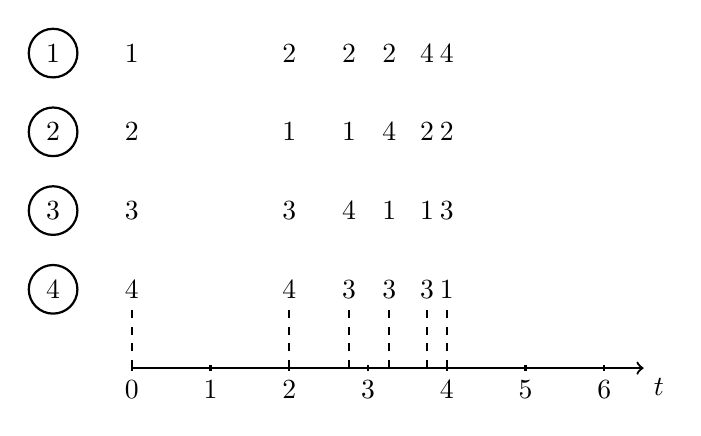
\begin{tikzpicture}[thick]
        \draw[thick,->] (0,0) -- (6.5,0) node[anchor=north west]
            {$t$};
%        \draw[thick,->] (0,0) -- (0,8) node[anchor=south east]
%            {valor$(t)$};
        \foreach \x in {0, 1,..., 6}
        \draw (\x cm,1pt) -- (\x cm,-1pt)
        node[anchor=north] {$\x$};
        \node[circle, draw] at (-1,1 cm) {$4$};
        \node[circle, draw] at (-1,2 cm) {$3$};
        \node[circle, draw] at (-1,3 cm) {$2$};
        \node[circle, draw] at (-1,4 cm) {$1$};

        \node at (0,1 cm) {$4$};
        \node at (0,2 cm) {$3$};
        \node at (0,3 cm) {$2$};
        \node at (0,4 cm) {$1$};

        \node at (2,1 cm) {$4$};
        \node at (2,2 cm) {$3$};
        \node at (2,3 cm) {$1$};
        \node at (2,4 cm) {$2$};

        \node at (2.76,1 cm) {$3$};
        \node at (2.76,2 cm) {$4$};
        \node at (2.76,3 cm) {$1$};
        \node at (2.76,4 cm) {$2$};

        \node at (3.27,1 cm) {$3$};
        \node at (3.27,2 cm) {$1$};
        \node at (3.27,3 cm) {$4$};
        \node at (3.27,4 cm) {$2$};

        \node at (3.75,1 cm) {$3$};
        \node at (3.75,2 cm) {$1$};
        \node at (3.75,3 cm) {$2$};
        \node at (3.75,4 cm) {$4$};

        \node at (4,1 cm) {$1$};
        \node at (4,2 cm) {$3$};
        \node at (4,3 cm) {$2$};
        \node at (4,4 cm) {$4$};


        \draw[dashed] (0, 0) -- (0, 0.8);
        \draw[dashed] (2, 0) -- (2, 0.8);
        \draw[dashed] (2.76, 0) -- (2.76, 0.8);
        \draw[dashed] (3.27, 0) -- (3.27, 0.8);
        \draw[dashed] (3.75, 0) -- (3.75, 0.8);
        \draw[dashed] (4, 0) -- (4, 0.8);


    \end{tikzpicture}
    \caption[Exemplo de trocas na lista ordenada]{Vetor com os índices dos elementos, ordenado
    pelos valores dos elementos no tempo $t = 0$ e suas
    alterações a medida que o tempo avança, para os quatro
    elementos da Figura~\ref{fig:ordenacao:exemplo}.}
    \label{fig:lista:vetores}
\end{figure}

Uma vez de posse do vetor ordenado com os valores iniciais
decrescentemente, construímos um certificado para cada par de
elementos consecutivos no vetor.
O $i$-ésimo certificado, denotado pelo par $(i, t)$, se refere ao par das posições $i$ e $i + 1$.
O valor $t$ consiste no instante de tempo em que o $i$-ésimo elemento
deixará de ter um valor maior que o valor do $(i + 1)$-ésimo
elemento do vetor, se esse instante for maior ou igual a 0, ou em
geral ao instante atual.
Do contrário, o valor $t$ consiste em $+\infty$.
O valor $t$ do certificado é o seu \textit{prazo de
validade}.

Esses prazos de validade determinam os \textit{eventos} que
potencialmente causarão modificações no vetor que mantém os
elementos ordenados pelo seu valor e, consequentemente, em alguns
certificados.

Esses $n - 1$ certificados são colocados em uma fila com
prioridades, com seu prazo de validade determinando a prioridade.
Estamos interessados nos certificados com menor prazo de validade.
Ou seja, a fila com prioridades pode ser implementada com um heap de
mínimo que usa os prazos de validade como chave.

Para descrever a implementação das três operações, precisamos
estabelecer o nome das variáveis usadas.
São elas:
\begin{enumerate}
    \item $n$: o número de elementos dados;
    \item $x_0$ e \textit{speed}: vetores com o valor e a velocidade
    inicial de cada um dos $n$ elementos;
    \item \now: instante atual.
    A variável \now\ será tratada como
    global, ou seja, será utilizada nas rotinas sem ser passada como
    argumento;
    \item \textit{sorted}: vetor com os índices dos $n$ elementos em
    ordem decrescente do seu valor no instante \textit{now};
%    \item \textit{indS}: vetor de $n$ posições; \textit{indS}[$j$]
%    guarda a posição em \textit{sorted} do elemento $j$;
    \item \textit{cert}: vetor com os $n-1$ certificados;
    \textit{cert}$[i]$ guarda o $i$-ésimo certificado, ou seja, o certificado
    entre $\sorted[i]$ e ${\sorted[i+1]}$, para~$1\leq i < n$;
    \item \textit{Q}: fila que guarda os inteiros $1, \ldots, n-1$,
    sendo \textit{cert}[$i$] a prioridade do inteiro $i$ na fila.
\end{enumerate}

\begin{figure}[H]
    \centering
    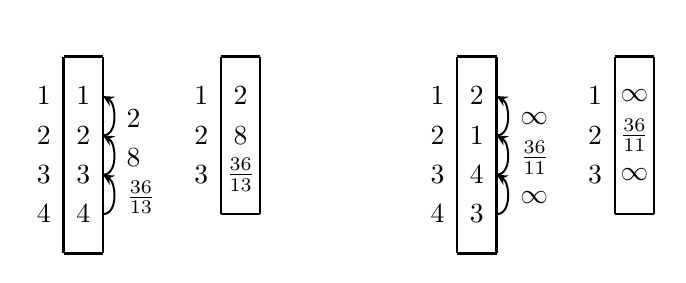
\begin{tikzpicture}[thick]
        \node at (0.5,0 cm) {$4$};
        \node at (0.5,0.5 cm) {$3$};
        \node at (0.5,1 cm) {$2$};
        \node at (0.5,1.5 cm) {$1$};

        \draw (0.75,-0.5) -- (0.75, 2);
        \draw (1.25,-0.5) -- (1.25, 2);
        \draw (0.75,-0.5) -- (1.25,-0.5);
        \draw (0.75, 2) -- (1.25, 2);
        \node at (1,0 cm) {$4$};
        \node at (1,0.5 cm) {$3$};
        \node at (1,1 cm) {$2$};
        \node at (1,1.5 cm) {$1$};

        \draw[->, shorten >= 0.1pt, shorten <= 0.1pt, >=stealth, line width=0.25mm]
        (1.25, 0) to[out=0,in=-30] node[right=1pt] {$\frac{36}{13}$} (1.25, 0.5);

        \draw[->, shorten >= 0.1pt, shorten <= 0.1pt, >=stealth, line width=0.25mm]
        (1.25, 0.5) to[out=0,in=-30] node[right=1pt] {$8$} (1.25, 1);

        \draw[->, shorten >= 0.1pt, shorten <= 0.1pt, >=stealth, line width=0.25mm]
        (1.25, 1) to[out=0,in=-30] node[right=1pt] {$2$} (1.25, 1.5);

        \node at (1,2.25 cm) {$\sorted$};

        \node at (2.5,0.5 cm) {$3$};
        \node at (2.5,1 cm) {$2$};
        \node at (2.5,1.5 cm) {$1$};

        \draw (2.75,0) -- (2.75, 2);
        \draw (3.25,0) -- (3.25, 2);
        \draw (2.75,0) -- (3.25,0);
        \draw (2.75, 2) -- (3.25, 2);
        \node at (3,0.5 cm) {$\frac{36}{13}$};
        \node at (3,1 cm) {$8$};
        \node at (3,1.5 cm) {$2$};

        \node at (3,2.25 cm) {$\cert$};

        \begin{scope}
            [shift={(5,0)}]
            \node at (0.5,0 cm) {$4$};
            \node at (0.5,0.5 cm) {$3$};
            \node at (0.5,1 cm) {$2$};
            \node at (0.5,1.5 cm) {$1$};

            \draw (0.75,-0.5) -- (0.75, 2);
            \draw (1.25,-0.5) -- (1.25, 2);
            \draw (0.75,-0.5) -- (1.25,-0.5);
            \draw (0.75, 2) -- (1.25, 2);
            \node at (1,0 cm) {$3$};
            \node at (1,0.5 cm) {$4$};
            \node at (1,1 cm) {$1$};
            \node at (1,1.5 cm) {$2$};

            \draw[->, shorten >= 0.1pt, shorten <= 0.1pt, >=stealth, line width=0.25mm]
            (1.25, 0) to[out=0,in=-30] node[right=1pt] {$\infty$} (1.25, 0.5);

            \draw[->, shorten >= 0.1pt, shorten <= 0.1pt, >=stealth, line width=0.25mm]
            (1.25, 0.5) to[out=0,in=-30] node[right=1pt] {$\frac{36}{11}$} (1.25, 1);

            \draw[->, shorten >= 0.1pt, shorten <= 0.1pt, >=stealth, line width=0.25mm]
            (1.25, 1) to[out=0,in=-30] node[right=1pt] {$\infty$} (1.25, 1.5);

            \node at (1,2.25 cm) {$\sorted$};

            \node at (2.5,0.5 cm) {$3$};
            \node at (2.5,1 cm) {$2$};
            \node at (2.5,1.5 cm) {$1$};

            \draw (2.75,0) -- (2.75, 2);
            \draw (3.25,0) -- (3.25, 2);
            \draw (2.75,0) -- (3.25,0);
            \draw (2.75, 2) -- (3.25, 2);
            \node at (3,0.5 cm) {$\infty$};
            \node at (3,1 cm) {$\frac{36}{11}$};
            \node at (3,1.5 cm) {$\infty$};

            \node at (3,2.25 cm) {$\cert$};

        \end{scope}
    \end{tikzpicture}
    \caption[Exemplo das estruturas utilizadas na lista ordenada]{Vetores $\sorted$ e $\cert$ para
        $\now = 0$ e $\now = 3$.
        O instante $t = \frac{36}{13}$ é quando as trajetórias dos elementos $3$ e $4$ se cruzam, e
        $t = \frac{36}{11}$ é quando as trajetórias dos elementos $1$ e $4$ se cruzam.}
    \label{fig:lista:variaveis}
\end{figure}



A interface da fila com prioridades que utilizaremos inclui as duas
seguintes operações:
\begin{enumerate}
    \item \textsc{minPQ}$(Q)$: devolve $i$ tal que
    \textit{cert}[$i$] é mínimo;
    \item \textsc{updatePQ}$(Q, i, t)$: altera a chave do
    $i$-ésimo certificado para $t$ e ajusta $Q$ de acordo.
\end{enumerate}

Note que não usaremos inserção ou remoção da fila com prioridades.

Para implementar a operação \textsc{change} de maneira eficiente, utilizaremos um vetor adicional
$\sorted$ que guarda em $\textit{indS}[j]$ a posição em $\sorted$ do elemento $j$.
Utilizaremos $\textit{indS}$ pois, dado um elemento $j$, precisamos saber a posição $i$ do
elemento $j$ em $\sorted$ para recalcular os certificados relacionados com a posição $i$.
Para implementar a operação \textsc{updatePQ}$(Q, i, t)$ em tempo logarítmico no número de
elementos na fila $Q$, é necessário utilizar um vetor adicional \textit{indQ} que guarda em
\textit{indQ}$[i]$ a posição em $Q$ do $i$-ésimo certificado.

Com isso, a operação \textsc{advance}$(t)$, implementada no
Algoritmo~\ref{alg:lista-ordenada:advance}, segue uma ideia bem simples: enquanto
$t$ for maior que o prazo de validade do próximo evento, avançamos
\textit{now} para esse prazo de validade e tratamos esse evento.
Nos problemas seguintes, a operação \textsc{advance}$(t)$ será essencialmente a
mesma;
as únicas mudanças ocorrerão no tratamento de um evento.

\begin{algorithm}[H]
    \caption[Algoritmo \textsc{advance}]{Função \textsc{advance}.} \label{alg:lista-ordenada:advance}
\begin{algorithmic}[1]
    \Function{advance}{$t$}
        \If{$t < $ \now}
            \State \Return
        \EndIf
        \State $i \leftarrow \Call{minPQ}{$Q$}$
        \While{$t \geq$ \cert[$i$]}
            \State \now $~\leftarrow$ \cert[i]
            \State $\Call{event}$
            \State $i \leftarrow \Call{minPQ}{$Q$}$
        \EndWhile
        \State \now $~\leftarrow$ $t$
    \EndFunction
\end{algorithmic}
\end{algorithm}

Um evento está associado a um certificado $(i, t)$ que expira quando
$\now = t$.
O tratamento do evento correspondente ao certificado $(i, t)$ consiste em trocar de lugar os
índices das posições $i$ e $i + 1$ do vetor \textit{sorted}, recalcular o prazo de validade do
$(i-1)$-ésimo certificado se $i > 1$, e do $(i + 1)$-ésimo
certificado se $i < n - 1$.
O $i$-ésimo certificado também deve ser ajustado para $+\infty$.
Finalmente, é necessário fazer ajustes em $Q$, nas chaves dos certificados que sofreram
alteração.

Na implementação da operação \textsc{event}, utilizaremos a rotina
\textsc{update}$(i)$ para calcular o novo prazo de validade $t$ do
$i$-ésimo certificado, se $1 \leq i < n$, e fazer os devidos ajustes
em~$Q$.
Para calcular $t$, utilizaremos uma rotina chamada \textsc{expire}$(i,
j)$, que calcula o prazo de validade dos certificados entre os
elementos $i$ e $j$ no instante \now.
A rotina auxiliar \textsc{expire}$(i, j)$ não mudará para outros problemas, mantendo a
mesma definição.
As implementações estão nos Algoritmos~\ref{alg:lista-ordenada:update}
e~\ref{alg:lista-ordenada:evento} e a Figura~\ref{fig:lista:expire}
ilustram as atualizações feitas por essas rotinas.

\begin{algorithm}
    \caption{Função \textsc{update}.} \label{lista:update}
\begin{algorithmic}[1]
    \Function{update}{$i$}
        \If{$1 \leq i < n$}
            \State $t \leftarrow $ \Call{expire}{$i,i+1$}
            \State \Call{updatePQ}{$Q,i,t$}
        \EndIf
    \EndFunction
\end{algorithmic}
\end{algorithm}

\begin{algorithm}
    \caption{Função \textsc{event}.} \label{torneioi:evento}
    \begin{algorithmic}[1]
        \Function{event}{\nnull}
            \State $e \leftarrow  $ \Call{minPQ}{$Q$}
            \While{$e.\cert$ = \now}
                \State $j \leftarrow e.\lastmatch$
                \State $k \leftarrow 2\cdot \floor{\frac{j}{2}}
                + ((j + 1)\mod2)$ \Comment{adversário}
                \While{$j > 1$ \AND \Call{compare}{$j, k$}}
                    \State \torneio[$\floor{\frac{j}{2}}$]
                    $\leftarrow~$\torneio[$j$]
                    \State $\torneio[k].\lastmatch$ $\leftarrow k$
                    \State \Call{update}{$\torneio[k]$}
                    \State $j \leftarrow \floor{\frac{j}{2}}$
                    \State $k \leftarrow 2\cdot \floor{\frac{j}{2}}
                    + ((j + 1)\mod2)$ \Comment{adversário}
                \EndWhile
                \State $\torneio[j].\lastmatch \leftarrow j$
                \State \Call{update}{$\torneio[j]$}
                \State $e \leftarrow  $ \Call{minPQ}{$Q$}
            \EndWhile
        % \LineComment{swapHeap$(i, \floor{\frac{i}{2}})$ troca \heap[$i$] por \heap$\left[\floor{\frac{i}{2}}\right]$}
        \EndFunction
        \LineComment{\Call{compare}{$i, j$} retorna se o valor
        de $i$ é maior que o valor de $j$.}
    \end{algorithmic}
\end{algorithm}

\begin{figure}[H]
    \centering
    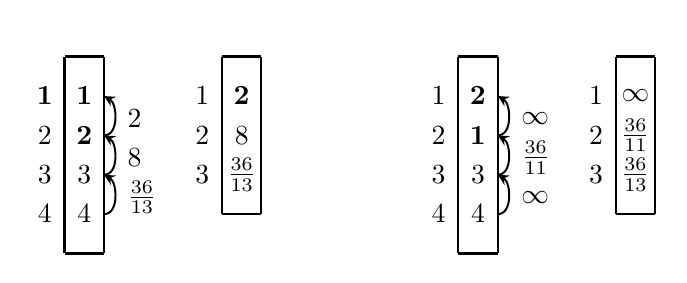
\begin{tikzpicture}[thick]
        \node at (0.5,0 cm) {$4$};
        \node at (0.5,0.5 cm) {$3$};
        \node at (0.5,1 cm) {$2$};
        \node at (0.5,1.5 cm) {\textbf{1}};

        \draw (0.75,-0.5) -- (0.75, 2);
        \draw (1.25,-0.5) -- (1.25, 2);
        \draw (0.75,-0.5) -- (1.25,-0.5);
        \draw (0.75, 2) -- (1.25, 2);
        \node at (1,0 cm) {$4$};
        \node at (1,0.5 cm) {$3$};
        \node at (1,1 cm) {$\textbf{2}$};
        \node at (1,1.5 cm) {$\textbf{1}$};

        \draw[->, shorten >= 0.1pt, shorten <= 0.1pt, >=stealth, line width=0.25mm]
        (1.25, 0) to[out=0,in=-30] node[right=1pt] {$\frac{36}{13}$} (1.25, 0.5);

        \draw[->, shorten >= 0.1pt, shorten <= 0.1pt, >=stealth, line width=0.25mm]
        (1.25, 0.5) to[out=0,in=-30] node[right=1pt] {$8$} (1.25, 1);

        \draw[->, shorten >= 0.1pt, shorten <= 0.1pt, >=stealth, line width=0.25mm]
        (1.25, 1) to[out=0,in=-30] node[right=1pt] {$2$} (1.25, 1.5);

        \node at (1,2.25 cm) {$\sorted$};

        \node at (2.5,0.5 cm) {$3$};
        \node at (2.5,1 cm) {$2$};
        \node at (2.5,1.5 cm) {$1$};

        \draw (2.75,0) -- (2.75, 2);
        \draw (3.25,0) -- (3.25, 2);
        \draw (2.75,0) -- (3.25,0);
        \draw (2.75, 2) -- (3.25, 2);
        \node at (3,0.5 cm) {$\frac{36}{13}$};
        \node at (3,1 cm) {$8$};
        \node at (3,1.5 cm) {$\textbf{2}$};

        \node at (3,2.25 cm) {$\cert$};

        \begin{scope}
            [shift={(5,0)}]
            \node at (0.5,0 cm) {$4$};
            \node at (0.5,0.5 cm) {$3$};
            \node at (0.5,1 cm) {$2$};
            \node at (0.5,1.5 cm) {$1$};

            \draw (0.75,-0.5) -- (0.75, 2);
            \draw (1.25,-0.5) -- (1.25, 2);
            \draw (0.75,-0.5) -- (1.25,-0.5);
            \draw (0.75, 2) -- (1.25, 2);
            \node at (1,0 cm) {$4$};
            \node at (1,0.5 cm) {$3$};
            \node at (1,1 cm) {$\textbf{1}$};
            \node at (1,1.5 cm) {$\textbf{2}$};

            \draw[->, shorten >= 0.1pt, shorten <= 0.1pt, >=stealth, line width=0.25mm]
            (1.25, 0) to[out=0,in=-30] node[right=1pt] {$\infty$} (1.25, 0.5);

            \draw[->, shorten >= 0.1pt, shorten <= 0.1pt, >=stealth, line width=0.25mm]
            (1.25, 0.5) to[out=0,in=-30] node[right=1pt] {$\frac{36}{11}$} (1.25, 1);

            \draw[->, shorten >= 0.1pt, shorten <= 0.1pt, >=stealth, line width=0.25mm]
            (1.25, 1) to[out=0,in=-30] node[right=1pt] {$\infty$} (1.25, 1.5);

            \node at (1,2.25 cm) {$\sorted$};

            \node at (2.5,0.5 cm) {$3$};
            \node at (2.5,1 cm) {$2$};
            \node at (2.5,1.5 cm) {$1$};

            \draw (2.75,0) -- (2.75, 2);
            \draw (3.25,0) -- (3.25, 2);
            \draw (2.75,0) -- (3.25,0);
            \draw (2.75, 2) -- (3.25, 2);
            \node at (3,0.5 cm) {$\frac{36}{13}$};
            \node at (3,1 cm) {$\bm{\frac{36}{11}}$};
            \node at (3,1.5 cm) {$\bm{\infty}$};

            \node at (3,2.25 cm) {$\cert$};

        \end{scope}
    \end{tikzpicture}
    \caption[Exemplo de expiração de certificado da lista ordenada]{No exemplo da
    Figura~\ref{fig:ordenacao:exemplo}, \cert[1] expirou no instante $\now = 2$, por isso
        $\sorted[1]$ e $\sorted[2]$ foram trocados e \cert[1] e \cert[2] foram atualizados.}
    \label{fig:lista:expire}
\end{figure}

A operação \textsc{query\_kth}$(i)$, implementada no Algoritmo~\ref{alg:lista:query}, consiste em
devolver \textit{sorted}$[i]$, enquanto que a operação \textsc{change}$(j, v)$ consiste em alterar
a posição $x_0[j]$ para $x_0[j] + (\textit{speed}[j] - v)\cdot now$,
a posição \textit{speed}[j] para \textit{v} e recalcular os
eventuais certificados de que $j$ participa.
O novo valor da posição $x_0[j]$ corresponde à posição inicial do elemento caso ele tivesse
começado com essa velocidade e estivesse na posição atual agora.
Além disso, a partir da posição $i$ em que $j$ se encontra no vetor
\textit{sorted}, podemos recalcular \textit{cert}$[i - 1]$ se $i >
1$ e \textit{cert}$[i]$ se $i < n$, como ilustrado na Figura~\ref{fig:lista:after}, acionando a
rotina \textsc{update} para fazer
os devidos acertos em~$Q$ correspondentes a estas modificações.
As instruções executadas pela operação \textsc{change} estão descritas
no Algoritmo~\ref{alg:lista-ordenada:change}.

\begin{algorithm}
    \caption{Função \textsc{query\_kth}.} \label{lista:query}
\begin{algorithmic}[1]
    \Function{query\_kth}{$i$}
        \If{$1 \leq i \leq n$}
            \State \Return \sorted[$i$]
        \EndIf
        \State \Return $-1$
    \EndFunction
\end{algorithmic}
\end{algorithm}

\begin{algorithm}
    \caption{Função \textsc{change}.} \label{torneioi:change}
    \begin{algorithmic}[1]
        \Function{change}{$j, v$}
            \State $e \leftarrow$ \Call{getObject}{$j$}
            \State $e.x_0 \leftarrow e.x_0+~(e.\speed -~v)~\cdot~\now$;
            \State $e.\speed \leftarrow v$
            \State $i \leftarrow e.\lastmatch$
            \State \Call{update}{$e$}
            \While{$i < n$}
                \If{$\torneio[i] = \torneio[2i]$}
                    \State $i \leftarrow 2i$
                \Else
                    \State $i \leftarrow 2i + 1$
                \EndIf
                \State $k \leftarrow 2\cdot \floor{\frac{i}{2}}
                + ((i + 1)\mod2)$ \Comment{adversário}
                \State \Call{update}{$\torneio[k]$}
            \EndWhile
        \EndFunction
    \end{algorithmic}
\end{algorithm}

\begin{figure}[H]
    \centering
    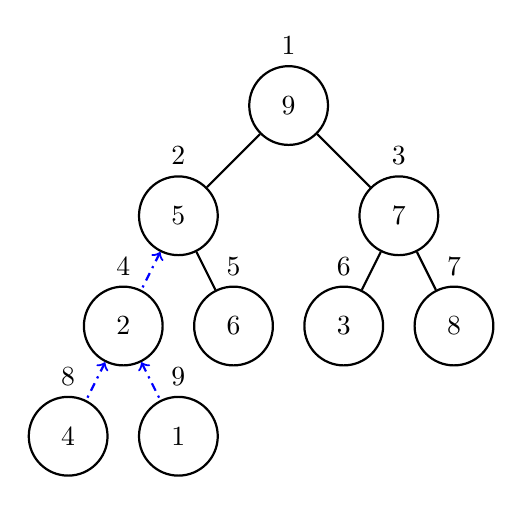
\begin{tikzpicture}[thick, scale=0.7]
        \node[label={1},circle,draw,minimum size=1cm]
        (1) at (0,0) {$9$};
        \node[label={2},circle,draw,minimum size=1cm]
        (2) at (-2,-2) {$5$};
        \node[label={3},circle,draw,minimum size=1cm]
        (3) at (2,-2) {$7$};
        \node[label={4},circle,draw,minimum size=1cm]
        (4) at (-3,-4) {$2$};
        \node[label={5},circle,draw,minimum size=1cm]
        (5) at (-1,-4) {$6$};
        \node[label={6},circle,draw,minimum size=1cm]
        (6) at (1,-4) {$3$};
        \node[label={7},circle,draw,minimum size=1cm]
        (7) at (3,-4) {$8$};
        \node[label={8},circle,draw,minimum size=1cm]
        (8) at (-4,-6) {$4$};
        \node[label={9},circle,draw,minimum size=1cm]
        (9) at (-2,-6) {$1$};

        \tikzstyle{cert}=[<-, dashdotted, blue, thick]
        \draw[thick] (1) -- (2);
        \draw[thick] (1) -- (3);
        \draw[cert] (2) -- (4);
        \draw[thick] (2) -- (5);
        \draw[thick] (3) -- (6);
        \draw[thick] (3) -- (7);
        \draw[cert] (4) -- (8);
        \draw[cert] (4) -- (9);
    \end{tikzpicture}
    \caption[Exemplo certificados do heap cinético após operação \textsc{change}]{Após a mudança de
    velocidade do elemento 2, que se encontra em \heap[$4$], os certificados
    \cert[$4$], \cert[$8$] e \cert[$9$] foram atualizados.}
    \label{fig:predeventheap}
\end{figure}

\subsection{Análise de desempenho}\label{subsec:analise-de-desempenho}

A lista ordenada cinética é uma estrutura \textit{responsiva}, pois o custo de
processar um certificado é exatamente o custo da rotina \textsc{event}, que é $O(\lg{n})$ pois a
rotina \textsc{update} consome $O(\lg{n})$ para atualizar a fila de prioridade dos certificados.

A lista ordenada cinética é uma estrutura \textit{eficiente}, pois todos os eventos
processados são eventos \textit{externos}, isto é, todo vencimento de
certificado representa a troca de ordem entre dois elementos na lista, que é uma
mudança na descrição combinatória do problema.

A lista ordenada cinética é uma estrutura \textit{compacta}, pois como cada
certificado está associado à relação de ordem entre um elemento e seu
predecessor, teremos no máximo $n-1$ certificados na fila de prioridades num
determinado instante.

A lista ordenada cinética é uma estrutura \textit{local}, pois cada elemento
está relacionado a no máximo dois certificados, o certificado entre ele e o
seu predecessor e o certificado entre o seu sucessor e ele.
